\chapter{Exemplo de aplicação}
Neste capítulo, descreveremos a construção de um simples aplicativo web para gerenciamento de tarefas. Mostraremos como acessar a API do Amazon SimpleDB usando a linguagem python e os resultados obtidos.

\section{Obtenção das chaves de acesso}
Primeiro deve-se criar uma conta na Amazon, cadastrando um cartão de crédito internacional para poder ter acesso aos serviços em nuvem da Amazon. Para acessar os serviços da AWS, é necessário fornecer identificadores de acesso durante a conexão. Em seguida, deve-se acessar a página \url{http://aws.amazon.com/} e, nas opções de conta, procurar por "Credenciais de Segurança"(figura 3.1).
\\
\begin{figure}
	\centering
	\fbox{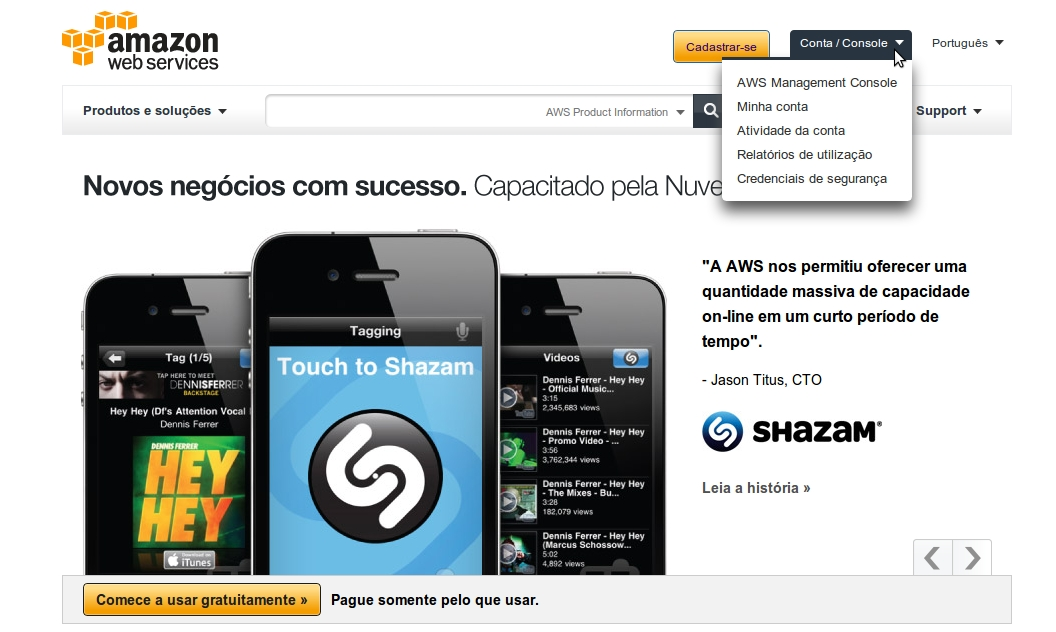
\includegraphics[scale=0.3]{figuras/acesso_credenciais.jpg}}
	\label{fig:acesso_credenciais}
	\caption{Credenciais de segurança}
\end{figure}
\\
Logo abaixo, na aba "Chaves de acesso", pode-se ver o ID de chave de acesso(figura 3.2) e a chave de acesso secreta(figura 3.3). Elas devem ser utilizadas pela aplicação para que ela possa acessar os serviços da Amazon.
\\
\begin{figure}
	\centering
	\fbox{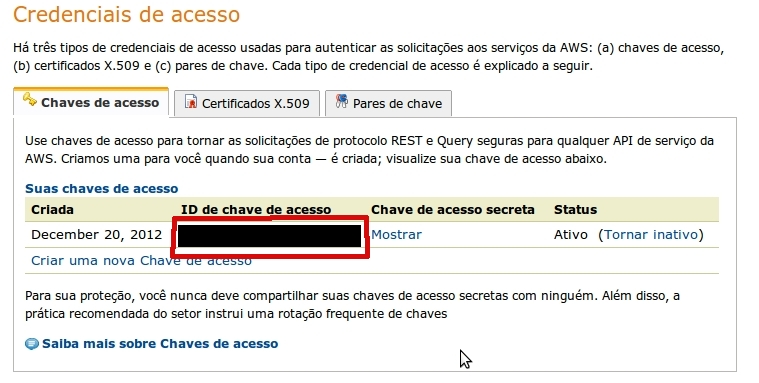
\includegraphics[scale=0.3]{figuras/credenciais1.jpg}}
	\label{fig:id_chave_acesso}
	\caption{ID de chave de acesso}
\end{figure}
\\
\\
\begin{figure}
	\centering
	\fbox{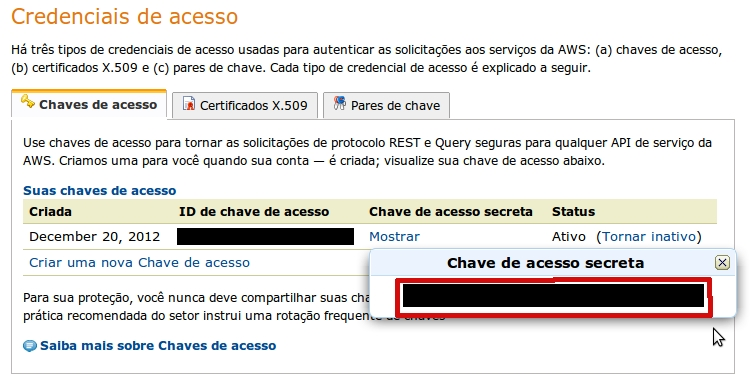
\includegraphics[scale=0.3]{figuras/credenciais2.jpg}}
	\label{fig:chave_acesso_secreta}
	\caption{Chave de acesso secreta}
\end{figure}